\documentclass[a4paper]{beamer}

\title{Idealised GFD Models III}
\author{Tim Leslie}\institute{Breakaway Consulting Pty. Ltd.\\Climate Change Research Centre}

\newcommand {\framedgraphic}[2] {
    \begin{frame}{#1}
        \begin{center}
            
        \end{center}
    \end{frame}
}

\begin{document}

\begin{frame}
\titlepage
\begin{columns}
    \begin{column}{0.25\textwidth}
      
\includegraphics[keepaspectratio]{CC-BY-SA.png}
    \end{column}
    \begin{column}{0.75\textwidth}
      This work is licensed under a \href{http://creativecommons.org/licenses/by-sa/3.0/}{Creative Commons Attribution-ShareAlike 3.0 Unported License}. Copyright 2012 Tim Leslie.
    \end{column}
\end{columns}
\end{frame}

\begin{frame}{Revision}
So far we have looked at
\begin{itemize}
\item The physical properties of fluids represented with equations
\item Simplifying equations based on further physical considerations
\item Numerical solving differential equations using a fixed time step
\item State variables, control parameters and dynamic coupling variables
\end{itemize}
\end{frame}

\begin{frame}{Field Valued Variables}
Consider the vorticity equation for a single ocean layer (eq (26) and (27) from Lecture I)
\begin{eqnarray}
q  &    =   & \frac{\nabla^2_Hp}{f_0} + \beta(y - y_0) + \frac{f_0}{H}\delta_z(\eta)\\
q_t & = & - \left(uq\right)_x - \left(vq\right)_y  -\frac{f_0}{H}\delta_z(e)+ A_2\frac{\nabla^4_Hp}{f_0}
\end{eqnarray}
The values of $u$, $e$, $p$ and $q$ are not just single values, but actually \emph{fields}.
\begin{eqnarray}
q(x,y)  &    =   & \frac{\nabla^2_Hp(x,y)}{f_0} + \beta(y - y_0) + \frac{f_0}{H}\delta_z(\eta)\\
q(x,y)_t & = & - \left(u(x,y)q(x,y)\right)_x - \left(v(x,y)q(x,y)\right)_y \nonumber\\
         &   & -\frac{f_0}{H}\delta_z(e(x,y))+ A_2\frac{\nabla^4_Hp(x,y)}{f_0}
\end{eqnarray}
\end{frame}

\begin{frame}{Spatial Discretisation}
\begin{itemize}
\item Even on a finite domain, there are an infinite number of points
\item We need to simplify our domain to contain a finite number of points for calculations
\item The more points, the more accurate the calculations can be.
\item The more points, the more calculations are needed per time step.
\item Tradeoff between \emph{resolution} and \emph{run time}.
\end{itemize}
\end{frame}

\begin{frame}{Numerical Grid}
The simplest way to choose our points is to place them on a rectangular grid
\begin{itemize}
\item A grid translates well to an array of numbers in a programming language
\item Spatial derivatives can be quickly computed
\item Data can be easily visualised
\end{itemize}
\end{frame}

\begin{frame}{Numerical differentiation}
Consider a field $f(x,y)$ on a rectangular grid, with the value at the grid point $(i,j)$ being $f_{i,j}$.
One way to compute $df/dx$ is
\begin{eqnarray}
\left(\frac{df}{dx}\right)_{i,j} & = & \frac{f_{i+1,j} - f_{i,j}}{\Delta x}
\end{eqnarray}
Another way is
\begin{eqnarray}
\left(\frac{df}{dx}\right)_{i,j} & = & \frac{f_{i+1,j} - f_{i-1,j}}{2\Delta x}
\end{eqnarray}
\end{frame}

\begin{frame}{Stencils}
Consider the points used in each of the previous calculations.
We call the pattern formed by these points the \emph{stencil}.
\begin{center}
  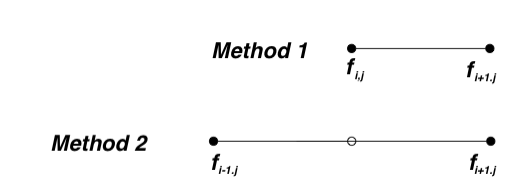
\includegraphics[width=\textwidth,height=0.5\textheight,keepaspectratio]{stencil1.png}
\end{center}
Using stencils to discuss algorithms is much easier than keeping track of indices.
\end{frame}

\begin{frame}{Laplacian Stencil}
Consider the following stencil
\begin{center}
  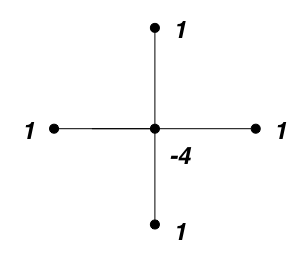
\includegraphics[width=\textwidth,height=0.3\textheight,keepaspectratio]{stencil2.png}
\end{center}
It tells us how to calculate the 5-point laplacian
\begin{eqnarray}
\nabla^2 f_{i,j}  & = & \frac{f_{i+1,j} + f_{i-1,j} + f_{i,j+1} + f_{i,j-1} - 4f_{i,j}}{\Delta^2}\\
                  & = & \left(\frac{f_{i+1,j} - 2f_{i,j} + f_{i-1,j}}{\Delta x^2}\right) +\left(\frac{f_{i,j+1} - 2f_{i,j} + f_{i,j-1}}{\Delta y^2}\right)\\
                  & = & \left(\frac{d^2f}{dx^2}\right)_{i,j} + \left(\frac{d^2f}{dy^2}\right)_{i,j}
\end{eqnarray}
\end{frame}

\begin{frame}{Sources of Numerical Error}
Whenever we do numerical calculations, errors will creep in.
\begin{itemize}
\item Physical measurement error
\item Floating point error
\item Discretisation error
\end{itemize}
\end{frame}

\begin{frame}{Physical Measurement Error}
Any input to the system we derives from a physical measurement will carry an error term.
\begin{itemize}
\item Initial state (Temperature, velocity, etc)
\item External forcing (Solar radiation, etc)
\item Physical parameters (density, heat capacity, etc)
\end{itemize}
Idealised models are less succeptible to these errors.
\end{frame}

\begin{frame}{Floating Point Error}
Computers store numbers using as floating point values. This means they can store a wide range of numbers (up to ~$10^310$x) but only with a finite precision.
\begin{itemize}
\item Numbers such as $\pi$, $\sqrt(2)$ get truncated, introducing an error.
\item Each calculation accumulates previous errors.
\item Floating point error typically begins around at 15 or 16 decimal places, but increases with time.
\end{itemize}
\end{frame}

\begin{frame}{Discretisation error}
Calculations such as spatial derivatives rely on approximations to the true value.
These are the main source of error in an idealised model
\begin{itemize}
\item Errors proportional to $\Delta$ or $\Delta^2$, depending on stencil used
\item Small $\Delta$ decreases errors but requires more computation.
\item Making $\Delta$ too small can (paradoxically) lead to non-realistic situations.
\end{itemize}
\end{frame}

\begin{frame}{CFL Condition}
If the fluid moves too fast and travels across multiple grid cells in a single time step, our numerical method becomes divergent.
\begin{itemize}
\item We compare to $u$ to $\frac{\Delta x}{\Delta t}$.
\item If we $u$ is too large (relatively), we say it violates the \emph{CFL condition}
\item If we make $\Delta x$ small to improve numerical accuracy, we must also make $\Delta t$ small to preserve the CFL condition.
\end{itemize}
\end{frame}

\begin{frame}{Summary}
In the past three lectures we have looked at idealised GFD models.
The key aspects of GFD modeling are
\begin{itemize}
\item Translating physical processes into mathematical statements.
\item Defining state variables, control parameters and coupling variables.
\item Using numerical methods to compute discrete values for the state variables.
\end{itemize}
\end{frame}

\end{document}
